\documentclass[11pt]{article}

\usepackage[margin=1in]{geometry}
\usepackage[T1]{fontenc}
\usepackage{mathptmx}
\usepackage[scaled=0.92]{helvet}
\usepackage{courier}
\usepackage{microtype}
\usepackage{amsmath,amssymb}
\usepackage{booktabs}
\usepackage{multirow}
\usepackage{graphicx}
\usepackage[table]{xcolor}
\usepackage{caption}
\usepackage{enumitem}
\usepackage{float}
\usepackage{tabularx}
\usepackage{needspace}
\usepackage[numbers,sort&compress]{natbib}
\usepackage[colorlinks=true,linkcolor=blue!50!black,citecolor=blue!50!black,urlcolor=blue!50!black]{hyperref}

\captionsetup{font=small,labelfont=bf}
\setlist{itemsep=2pt,topsep=4pt}
\newcommand{\todo}[1]{\textcolor{red!70!black}{[#1]}}
\newcommand{\ci}[2]{\,[#1,\,#2]}

\title{When Does Brier-Reward RL Help a Small Language Model Forecast?\\
\large Controlled Experiments on Kalshi Economic Markets}
\author{Anirudh Srikanth\\University of Pennsylvania\\\texttt{anirudh1@engineering.upenn.edu}}
\date{October 2026}

\begin{document}
\maketitle

\begin{abstract}
We study whether reinforcement learning with a Brier-score reward improves how a small language model uses fixed forecasting evidence. We train Llama~3.2~3B Instruct with GRPO on 1,391 resolved Kalshi questions about scheduled U.S.\ economic releases; each prompt supplies only the series' recent results, all public before the question was asked. Listed plainly, these results give the untrained model little discrimination (validation AUC 0.52, against 0.85 for a counting rule over the same numbers); a deterministic block stating the threshold comparisons raises it to 0.76. With this block and GRPO's group-standard-deviation scaling disabled, three training seeds improved both Brier score and AUC. On a later test split of 479 questions in 13 announcement clusters, the model comparisons met their precommitted criteria: against the untrained model with the same prompt, Brier changed by $-0.025$ (95\% interval $-0.034$ to $-0.016$) and AUC by $+0.033$ ($+0.018$ to $+0.054$), and these runs beat the runs with the scaling enabled in log loss and calibration error. With the scaling enabled, all three seeds collapsed onto a latest-result heuristic, answering almost only 0 or 1 on validation and test questions, although a calibrated version of that heuristic earns a higher Brier reward. With the scaling disabled, the plain-prompt and shuffled-outcome runs contracted toward a constant. The trained models did not outperform a logistic regression or gradient-boosted trees on the supplied features. Under our one-pass training budget, only the structured prompt with std scaling disabled showed supported improvements in both Brier score and AUC. All experiments ran on free Kaggle T4 GPUs, about 30 GPU-hours in total.
\end{abstract}

\section{Introduction}

Several groups now train language models to forecast with reinforcement learning, rewarding them with a proper scoring rule on questions whose outcomes are known \citep{turtel2025outcome,turtel2026proper,chandak2025scaling,afifi2026research,ye2026alphabet,han2026futureworld}. The headline metric is usually the Brier score, and it usually improves. But a Brier score improvement can come from different sources. It can come from correcting the average probability without improving the ordering of the forecasts \citep{vancalster2016hierarchy}. The spread of the forecasts can change. Or the model can put higher probabilities on the questions that resolve YES, which is discrimination; we measure it separately with AUC. Most of these systems also retrieve news or search the web, so a gain can come from better searching, better reading or better forecasting. Among the forecasting studies we reviewed, one reports discrimination for the trained model. There, a Brier reward improved the Brier score from 0.186 to 0.165 but AUC only from 0.725 to 0.751 \citep{turtel2026proper}.

We ask a narrower question in a setting built to answer it: \emph{with the evidence held fixed, does proper-score RL improve how a small model uses that evidence?} Kalshi's markets on scheduled economic releases suit this well. Most questions have a numeric threshold (``Will CPI rise by more than 0.3\% in May?''); the exception is the Fed's rate decision (cut, hold or hike). Every series has a history of comparable past results. That history lets us build the evidence from public data with settlement timestamps, so nothing the model sees postdates the question. It also lets us write simple rules over the same evidence as baselines, and the market price at question time gives a strong external benchmark that the model never sees.

We train Llama~3.2~3B Instruct \citep{grattafiori2024llama3} with GRPO \citep{shao2024deepseekmath} and a Brier reward on 1,391 questions from 2024 and 2025, and evaluate on 410 questions from 2026. Ten training runs cross two prompts with two settings of GRPO's advantage scaling, repeat the key-numbers conditions over three seeds, and add a shuffled-outcome control. Our main findings on the validation split:

\begin{enumerate}[leftmargin=*]
\item \textbf{The plain prompt elicits little discrimination; stating the comparisons explicitly substantially improves it.} With six recent results in the prompt, the untrained model has Brier 0.272, worse than the constant-0.5 baseline's 0.250, and near-chance AUC of 0.52, while a counting rule over the same numbers reaches AUC 0.85. A deterministic ``key numbers'' block raises the untrained model's AUC to 0.76. An ablation traces the gain mainly to restating the YES condition and counting the recent results that would have resolved YES (\S\ref{sec:elicitation}).
\item \textbf{Among the configurations tested, only the key-numbers prompt with std scaling disabled improved both Brier score and AUC} under our one-pass training budget: $-0.031$ and $+0.070$ averaged over three seeds (test: $-0.025$ and $+0.033$), with no detectable change in calibration error. With outcomes shuffled, the same setup gets worse, so the improvement depends on the real association between inputs and outcomes (\S\ref{sec:twobytwo}).
\item \textbf{With GRPO's default scaling, RL collapses onto a lookup rule.} In all three seeds, the share of near-certain answers passes 90\% within about 140 steps. More than 98\% of evaluation answers end up exactly 0 or 1, on validation and on test, matching a one-cue rule: ``1 if the latest result already satisfies the question, else 0.'' Under the training reward itself, this rule scores worse than the same rule stated at its hit rates (average Brier term 0.847 vs 0.870, excluding the $+0.5$ format bonus that every readable answer gets). \citet{bereket2025uncalibrated} identified this overconfidence from std scaling and showed that removing it corrects it. We add its appearance with a Brier reward on real economic forecasting questions, its interaction with how the evidence is presented, and collapse onto an identifiable heuristic in every seed (\S\ref{sec:collapse}).
\item \textbf{The trained models do not outperform simple models on the same features.} The best runs neither beat nor clearly trail a logistic regression on five key-number features and the counting rule (intervals include 0). They trail gradient-boosted trees on AUC by 0.03 to 0.04 on validation; on the test split that gap is smaller and not resolved. The market is far ahead of everything, with Brier 0.062 (\S\ref{sec:simple}).
\end{enumerate}
On a later test split, scored once against precommitted model comparisons, the predictions for findings 2 and 3 all held, and findings 1 and 4 were repeated as descriptive comparisons (\S\ref{sec:test}). Two boundaries round these out. With std scaling disabled, the plain-prompt and shuffled-outcome runs contract toward a constant, consistent with hedging when no usable signal is used (\S\ref{sec:twobytwo}). And we find no useful discrimination on held-out weather brackets under this evidence setup (\S\ref{sec:weather}).

Methodologically, we report AUC and a shift-matched baseline next to every Brier score. Intervals resample whole announcements, since series released together resolve together. Every model is compared with simple rules built from its own prompt. On the test split, the model comparisons were committed to the repository before any language model was scored on it (Appendix~\ref{app:timeline} gives the timeline). Code, prompts, per-question answers and the reward-hacking log are public.\footnote{\url{https://github.com/anisrikanth/calibrated-forecasting-rl}}

\section{Related work}

\paragraph{RL for language-model forecasting.} \citet{turtel2025outcome} train a 14B reasoning model with GRPO-family algorithms and a Brier-type reward on Polymarket questions with retrieved news. They report that plain GRPO made 39\% of forecasts extreme. \citet{turtel2026proper} compare five proper scoring rules on a 120B model without std scaling, and report AUC and a bias--information--noise decomposition \citep{satopaa2021bin}. \citet{chandak2025scaling}, \citet{afifi2026research}, \citet{ye2026alphabet} and \citet{han2026futureworld} train models from 3B to over 100B parameters with search or retrieved news. \citet{levy2025rl} trains 1.5B to 7B models against market prices and outcomes. Two hedging failures resemble ours. A Brier-only reward led \citet{chandak2025scaling}'s model to answer ``Unknown'' about 40\% of the time, and training on outcomes collapsed \citet{levy2025rl}'s model to always saying 50\%. Our setting differs in holding the evidence fixed and small (six numbers), so that what RL changes can be measured against rules over the same numbers.

\paragraph{Forecasting benchmarks and markets.} LLM forecasters approach but do not reach human crowds and markets \citep{halawi2024approaching,karger2025forecastbench,zou2022autocast}. Live and market-based benchmarks are now common \citep{zeng2026futurex,yang2025prophetarena,nel2025kalshibench}, and small untrained models often lose to the base rate \citep{li2026canllms}. Kalshi's macro markets are as accurate as consensus forecasts and futures, or more so \citep{diercks2026kalshi}. Low-priced Kalshi contracts are overpriced \citep{burgi2026makers}, which matters mostly for our weather brackets.

\paragraph{Training stated confidence.} Supervised fine-tuning can teach a model to state calibrated probabilities for its own answers \citep{lin2022teaching}, and models already trained with human feedback state better-calibrated confidence under suitable prompts \citep{tian2023just}. RLHF itself tends to make stated confidence overconfident, which calibrating the reward model reduces \citep{leng2025taming}. Training directly with a proper scoring rule as the reward also improves calibration \citep{baniharouni2026rewarding,damani2026beyond}, and in one study discrimination too: with a log-score reward, Llama~3 8B's AUROC on TriviaQA rose from 0.59 to 0.86 \citep{baniharouni2026rewarding}. There the signal, whether the model knows the answer, is already inside the model. In our setting it has to be read from the prompt.

\paragraph{What GRPO changes.} GRPO scores each answer against the other answers to the same question \citep{shao2024deepseekmath}. Its normalizations bias training \citep{liu2025understanding}. \citet{bereket2025uncalibrated} show that, with a log-score reward on stochastic yes/no outcomes, dividing by the group's standard deviation drives forecasts to the extremes, while PPO, RLOO and GRPO without the division do not. RL for reasoning mostly sharpens what the base model already samples \citep{yue2025doesrl}, and even random rewards can change behaviour through GRPO's clipping \citep{shao2026spurious}. That motivates our shuffled-outcome control.

\paragraph{Language models and numbers.} LLMs can extrapolate numeric sequences \citep{gruver2023llmtime} but make basic comparison errors \citep{yang2025numbercookbook}. Removing the LLM from LLM-based time-series forecasters often does not hurt \citep{tan2024useful}, so we report simple rules and supervised models in every table.

\paragraph{Evaluating forecasters.} Questions that resolve together share drivers, so effective sample sizes are far below question counts \citep{paleka2025pitfalls}. We therefore resample whole announcements. We use the Brier score \citep{brier1950verification}, proper scoring rules \citep{gneiting2007strictly}, and the ladder consistency checks of \citet{paleka2025consistency}.

\section{Setup}
\label{sec:setup}

\subsection{Data}

We pull every resolved market from eight Kalshi economic series, January 2024 to October 2026. The series are month-over-month and year-over-year CPI, both headline and core; nonfarm payrolls; the unemployment rate; the Fed funds rate after each meeting; and the Fed's rate decision (cut, hold or hike, by size). We use three units:
\begin{itemize}[leftmargin=*]
\item A \emph{question} is one threshold market (``CPI rises by more than 0.2\%'').
\item A \emph{release} is one series' ladder of thresholds for one data point; this is Kalshi's ``event''.
\item An \emph{announcement} is everything published together: CPI's four series come out in one release, payrolls and unemployment share the jobs report, and the Fed rate and decision share a meeting.
\end{itemize}
The data contain 2,296 questions in 249 releases.

\paragraph{Timing.} Every question is asked exactly 24 hours before its market closes; none needed shifting to fit a market's opening time. Markets close at the scheduled announcement: 8:25 to 8:30 Eastern for CPI and the jobs report, and just before the 2~pm Fed statement. Four validation releases close shortly after the announcement, on the same morning. So every question comes about a day before the announcement it is about. The only markets that settled long after closing are training questions whose releases the 2025 government shutdown delayed; those markets closed before the delayed release. A question's evidence is the six most recent results of the same series whose markets \emph{settled} strictly before the question time, read from Kalshi's settlement values. Settlement follows the public release, so this is conservative, and an audit finds no context entry settled at or after its question.

\paragraph{Splits.} We split by release date, keeping every threshold of a release, and every release closing on the same day, in one split:
\begin{itemize}[leftmargin=*]
\item \emph{Training:} the oldest 70\% of releases (177 releases, 1,391 questions, January 2024 to December 2025, yes-rate 0.491).
\item \emph{Validation:} the next 15\% (36 releases, 13 announcements, 410 questions, January to May 2026, yes-rate 0.461).
\item \emph{Test:} the newest 15\% (36 releases, 13 announcements, 495 questions, June to October 2026).
\end{itemize}
All development decisions used the validation split; the language models are scored on the test split once, against precommitted comparisons (\S\ref{sec:test}). The baselines' test scores were computed earlier, while the evaluation code was being tested (Appendix~\ref{app:timeline}). As an out-of-domain set we use daily high-temperature brackets for New York and Chicago. They are never trained on; we score 60 city-days sampled from 2026 (56 dates, 360 questions; yes-rate 0.167).

\paragraph{Contamination and leakage.} These are two separate issues. Pretraining contamination: Llama~3.2 was released in September 2024 with a stated knowledge cutoff of December 2023, and all evaluation questions are from 2026, so fixed weights released earlier cannot contain their outcomes. Some 2024 training outcomes predate the model's release, which affects what the model trains on, not how it is evaluated. Pipeline leakage: the timing audit above covers it.

\paragraph{Benchmark.} As a benchmark we take the market price at question time, from the last hourly candle before it (the bid--ask midpoint if the spread is at most 0.20, otherwise the last trade). The model never sees it. All methods are scored on the questions that have a price: all 410 in validation, and 479 of the 495 test questions (yes-rate 0.409).

\subsection{Prompts}

The system prompt asks for brief reasoning and a final line \texttt{Probability: 0.XX} (Appendix~\ref{app:prompt}). The user message gives the date, the market's resolution rule as the question, and the recent results, oldest first. We call this the \textbf{plain} prompt. The \textbf{key-numbers} prompt adds a deterministic block computed from the same inputs, with five lines:
\begin{enumerate}[leftmargin=*]
\item the YES condition in plain words;
\item the latest result and its distance from the threshold;
\item the change from the result before;
\item how many recent results would have resolved YES;
\item the recent average and range.
\end{enumerate}
The block contains no new observations. It supplies engineered comparisons and counts over the same data, and that change in representation is the intervention we study. Fed-decision questions have no numeric threshold and get no block.

\subsection{Training}

We train LoRA adapters \citep{hu2022lora} (rank 32, $\alpha=32$, all attention and MLP projections; 48.6M trainable parameters) with TRL's GRPO trainer \citep{vonwerra2020trl} and Unsloth \citep{unsloth}, sampling answers with vLLM \citep{kwon2023vllm}. Each question gets 4 sampled answers, and each step uses 4 questions. One pass over the training questions is 347 steps. We use learning rate $10^{-5}$ with cosine decay and 10\% warm-up, no KL penalty, and TRL's default token-level (DAPO) loss \citep{yu2025dapo}; full settings are in Appendix~\ref{app:hyper}.

The reward for an answer depends on whether it ends with a readable probability $p$. With $y \in \{0,1\}$ the question's outcome, a readable answer gets $1-(p-y)^2 + 0.5$, which lies between 0.5 and 1.5. An unreadable answer gets $-1$. When all four answers to a question are readable, the $+0.5$ is shared by every answer in the group and cancels in the advantages. Unreadable answers were 5\% to 13\% of each run's first 512 training answers and at most 0.4\% of its last 512.

GRPO's advantage for answer $i$ in a group of $G=4$, writing $\bar r$ for the group's average reward and $\operatorname{std}(r)$ for its standard deviation, is
\[
A_i^{\text{std on}} = \frac{r_i - \bar r}{\operatorname{std}(r) + \epsilon} \qquad\text{or}\qquad A_i^{\text{std off}} = r_i - \bar r .
\]
The first is TRL's default (\texttt{scale\_rewards="group"}). The second removes the division, as in Dr.\ GRPO \citep{liu2025understanding}. Removing it does not make the full clipped procedure an unbiased estimator; it only removes the per-group rescaling. Table~\ref{tab:runs} lists the runs.

\begin{table}[t]
\centering\small
\caption{Training runs. All use Llama~3.2~3B Instruct, LoRA rank 32, a Brier plus format reward, 4 answers per question and 4 questions per step. The seed is the training seed (LoRA initialisation, question order and training samples); evaluation sampling uses the same seed in every run.}
\label{tab:runs}
\begin{tabular}{lllll}
\toprule
Run & Prompt & Std scaling & Training & Seed \\
\midrule
1 & Plain & On & 1 pass, lr $10^{-5}$ & 3407 \\
2 & Plain & On & 2 passes, lr $2\times10^{-5}$ & 3407 \\
7 & Plain & Off & 1 pass, lr $10^{-5}$ & 3407 \\
3, 9, 10 & Key numbers & On & 1 pass, lr $10^{-5}$ & 3407, 1, 2 \\
4, 5, 6 & Key numbers & Off & 1 pass, lr $10^{-5}$ & 3407, 1, 2 \\
8 & Key numbers & Off & 1 pass, lr $10^{-5}$, outcomes shuffled & 3407 \\
\bottomrule
\end{tabular}
\end{table}

\subsection{Evaluation}

Each model answers each question 4 times (temperature 0.7, top-$p$ 0.95, at most 320 tokens, fixed seed). Its forecast is the average of the readable answers, or 0.5 if none is readable. Every trained run's validation answers were all readable; the untrained models' were 97.7\% to 98.4\% readable. Counting each unreadable answer as 0.5 instead changes no Brier score by more than 0.002. We report:
\begin{itemize}[leftmargin=*]
\item the Brier score;
\item log loss, with probabilities clipped to $[0.01, 0.99]$;
\item calibration error (ECE, 10 equal-width bins);
\item AUC: the chance that a random YES question gets a higher forecast than a random NO question, with ties counting half; it ignores the level of the forecasts.
\end{itemize}
The primary estimand is performance on a randomly chosen listed question, so announcements with more thresholds carry more weight. Equal-announcement weighting is reported as a check (Appendix~\ref{app:diag}).

Every comparison is paired on the same questions. Its 95\% interval comes from 4,000 bootstrap draws that resample whole announcements, since all thresholds of all series released together resolve together \citep{paleka2025pitfalls}. Validation and test each contain 13 announcement clusters, so the intervals are rough. They account for dependence within announcements but may not capture dependence across time: successive announcements share economic conditions and overlapping recent results. Resampling single releases instead gives very similar intervals (Appendix~\ref{app:diag}). For groups of runs (three seeds), each draw averages the group's runs on the same resampled announcements. These are paired cluster-bootstrap intervals for the trained models we observed. They cover question sampling, not variation across training seeds, so we report each seed's result and the range across seeds separately.

\paragraph{Baselines on the same evidence.} All are fitted on the training questions only; Appendix~\ref{app:baselines} gives the exact feature definitions.
\begin{itemize}[leftmargin=*]
\item \emph{Base rate:} each series' training yes-rate.
\item \emph{Counting rule:} the share of the six recent results that would have resolved YES.
\item \emph{Latest-result rule:} 1 if the latest result already would have, else 0.
\item \emph{Logistic regression:} five features from the key numbers, with an L2 penalty.
\item \emph{Gradient-boosted trees:} the same five features, with and without the series as a categorical feature. Settings are chosen by cross-validation on the training questions, with each announcement kept in one fold.
\end{itemize}
Questions without a threshold get the base rate. We also report a \emph{shift-matched} untrained model, moved up or down to the trained model's average forecast. It has a narrow purpose: to show when a Brier gain could come from moving the average alone. It is not a test against every possible recalibration.

\section{Results}

\begin{table}[t]
\centering\small
\caption{Every method on the 410 validation econ questions (36 releases, 13 announcements; yes-rate 0.461). Four-answer averages. For the two groups of three seeds we show the average and, in brackets, the range across seeds. Bold: the best Brier score, log loss and AUC short of the market. Paired comparisons with intervals are in Tables~\ref{tab:twobytwo} and~\ref{tab:boot}.}
\label{tab:main}
\setlength{\tabcolsep}{4pt}
\begin{tabular}{lcccc}
\toprule
Method & Brier $\downarrow$ & Log loss $\downarrow$ & ECE $\downarrow$ & AUC $\uparrow$ \\
\midrule
Market price (never shown to the model) & 0.062 & 0.200 & 0.023 & 0.977 \\
\midrule
Gradient-boosted trees, key numbers + series & \textbf{0.151} & \textbf{0.468} & 0.062 & \textbf{0.869} \\
Gradient-boosted trees, key numbers & 0.159 & 0.487 & 0.089 & 0.859 \\
Logistic regression, key numbers & 0.163 & 0.522 & 0.087 & 0.855 \\
Counting rule & 0.168 & 0.573 & 0.121 & 0.846 \\
Latest-result rule (0/1) & 0.218 & 1.003 & 0.212 & 0.775 \\
Base rate & 0.243 & 0.679 & 0.042 & 0.577 \\
Always 0.5 & 0.250 & 0.693 & 0.039 & 0.500 \\
\midrule
Untrained, plain prompt & 0.272 & 0.748 & 0.120 & 0.520 \\
Run 1: plain, std on & 0.267 & 0.734 & 0.123 & 0.544 \\
Run 2: plain, std on, 2 passes, lr $2\times10^{-5}$ & 0.320 & 1.287 & 0.298 & 0.686 \\
Run 7: plain, std off & 0.263 & 0.720 & 0.107 & 0.485 \\
\midrule
Untrained, key numbers & 0.201 & 0.594 & 0.060 & 0.757 \\
Untrained, best three key-number lines (ablation) & 0.190 & 0.564 & 0.055 & 0.789 \\
Runs 3, 9, 10: key numbers, std on & 0.219 {\scriptsize[.211, .223]} & 0.990 {\scriptsize[.93, 1.03]} & 0.216 {\scriptsize[.21, .22]} & 0.782 {\scriptsize[.77, .80]} \\
Runs 4, 5, 6: key numbers, std off & 0.170 {\scriptsize[.169, .171]} & 0.522 {\scriptsize[.52, .53]} & 0.068 {\scriptsize[.05, .09]} & 0.827 {\scriptsize[.82, .83]} \\
Run 8: key numbers, std off, shuffled outcomes & 0.236 & 0.665 & 0.113 & 0.708 \\
\bottomrule
\end{tabular}
\end{table}

\subsection{The plain prompt elicits little discrimination}
\label{sec:elicitation}

With the plain prompt, the untrained 3B model scores Brier 0.272 and AUC 0.520 (Table~\ref{tab:main}). Its Brier score is worse than always saying 0.5 (0.250), and worse than its own with the recent results removed (0.253). The evidence itself is usable: the counting rule over the same six numbers scores 0.168 and AUC 0.846. The model's reasoning and its final probability often disagree, and 48\% of adjacent threshold pairs in a ladder are ordered the wrong way (Appendix~\ref{app:diag}).

The key-numbers block raises the untrained model's AUC from 0.520 to 0.757 (+0.237, interval +0.189 to +0.312) and lowers its Brier score to 0.201, the first model setting to beat the base rate. Figure~\ref{fig:ablation} reveals the block one line at a time, still with no training. The intervals below resample announcements.
\begin{itemize}[leftmargin=*]
\item \textbf{Restating the YES condition alone} raises AUC by 0.093 (+0.038 to +0.147). Part of the failure is parsing Kalshi's legal-style rule text.
\item \textbf{Adding the latest result against the threshold} raises AUC a further 0.059 ($-0.005$ to $+0.131$), not resolved at this sample size.
\item \textbf{Adding the count of recent results that would have resolved YES} raises it a further 0.117 (+0.054 to +0.194). These three lines give the best untrained prompt: Brier 0.190, AUC 0.789, ECE 0.055.
\item \textbf{The change and range lines add nothing detectable.} Against the three-line version, the full block's AUC is 0.030 lower ($-0.006$ to $+0.064$).
\item \textbf{The YES condition plus the count, without the latest result,} scores below the full block (AUC $-0.048$, $-0.094$ to $+0.011$), but the difference is not resolved.
\item \textbf{Asking the model to estimate the number first does not help.} With the plain context, ``estimate the value, then compare it with the threshold'' scores the same as the plain prompt (AUC 0.522, change $+0.003$, $-0.065$ to $+0.073$), and 8\% of its answers lose the probability line.
\end{itemize}
The ablation supports a representation-and-comparison bottleneck. The estimate-first prompt we tested did not improve performance.

\begin{figure}[t]
\centering
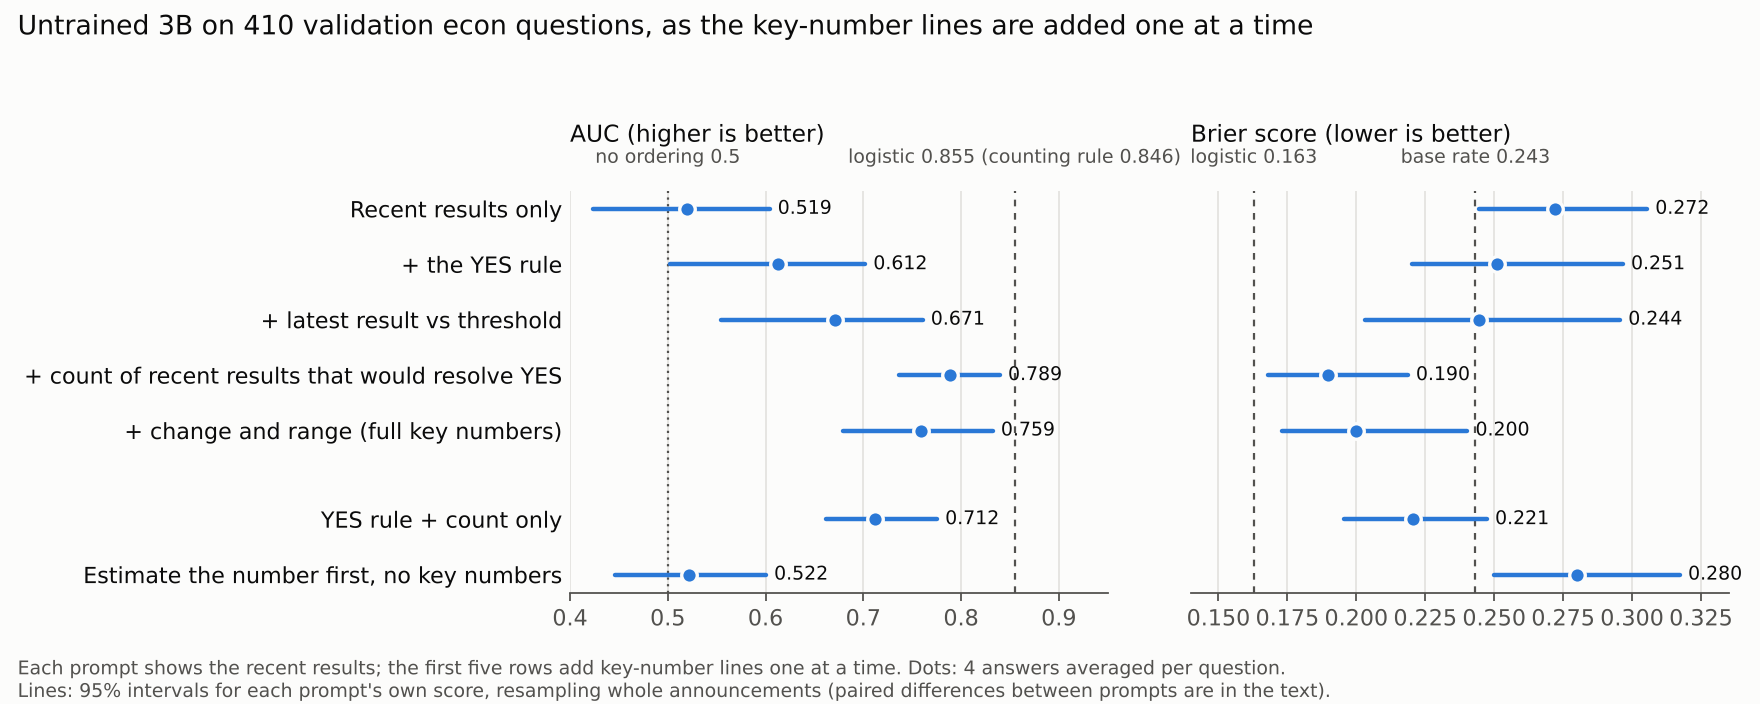
\includegraphics[width=\linewidth]{figures/prompt_ablation.png}
\caption{Untrained model, validation econ questions: AUC and Brier score as the key-numbers block is revealed one line at a time (top five rows), and two alternatives. Lines are 95\% intervals for each prompt's own score, resampling whole announcements; paired differences between prompts are given in the text. The ablation is its own generation batch: its full-block row (AUC 0.759, Brier 0.200) differs slightly from the untrained key-numbers model in Table~\ref{tab:main} (0.757, 0.201), which comes from an earlier batch with the same prompt and sampling seed (88\% of answers identical). Comparisons among the ablation's prompts use the ablation batch; all other comparisons with the untrained model use the earlier batch.}
\label{fig:ablation}
\end{figure}

\subsection{Prompt and std scaling}
\label{sec:twobytwo}

Table~\ref{tab:twobytwo} crosses the two prompts with the two settings of GRPO's advantage scaling. Figure~\ref{fig:spread} shows how the spread of stated probabilities evolves during training in each cell. The plain-prompt cells have one seed each.

\begin{table}[t]
\centering\small
\caption{The four prompt-by-scaling conditions on validation econ: Brier / AUC, and the change from the untrained model with the same prompt (95\% interval, resampling announcements). The key-numbers cells average three seeds each; the plain-prompt cells are single runs.}
\label{tab:twobytwo}
\begin{tabular}{p{2.6cm}p{5.6cm}p{5.6cm}}
\toprule
 & GRPO std scaling on & GRPO std scaling off \\
\midrule
Plain prompt \newline {\scriptsize untrained 0.272 / 0.520} & Run 1: 0.267 / 0.544. Average forecast falls by 0.06; Brier $-0.005$ \ci{-0.024}{+0.017}, AUC $+0.024$ \ci{-0.027}{+0.075}. & Run 7: 0.263 / 0.485. Forecasts contract toward 0.56 (spread 0.17 $\to$ 0.06); Brier $-0.009$ \ci{-0.029}{+0.007}, AUC $-0.035$ \ci{-0.085}{+0.013}. \\
\addlinespace
Key numbers \newline {\scriptsize untrained 0.201 / 0.757} & Runs 3, 9, 10: 0.219 / 0.782. Collapse to 0/1 copies of the latest-result rule; Brier $+0.017$ \ci{-0.032}{+0.074}, log loss $+0.396$ \ci{+0.142}{+0.690}. & \textbf{Runs 4, 5, 6: 0.170 / 0.827.} Brier $\mathbf{-0.031}$ \ci{-0.045}{-0.016}, AUC $\mathbf{+0.070}$ \ci{+0.036}{+0.119}, ECE $+0.008$ \ci{-0.024}{+0.039}. \\
\bottomrule
\end{tabular}
\end{table}

\begin{figure}[t]
\centering
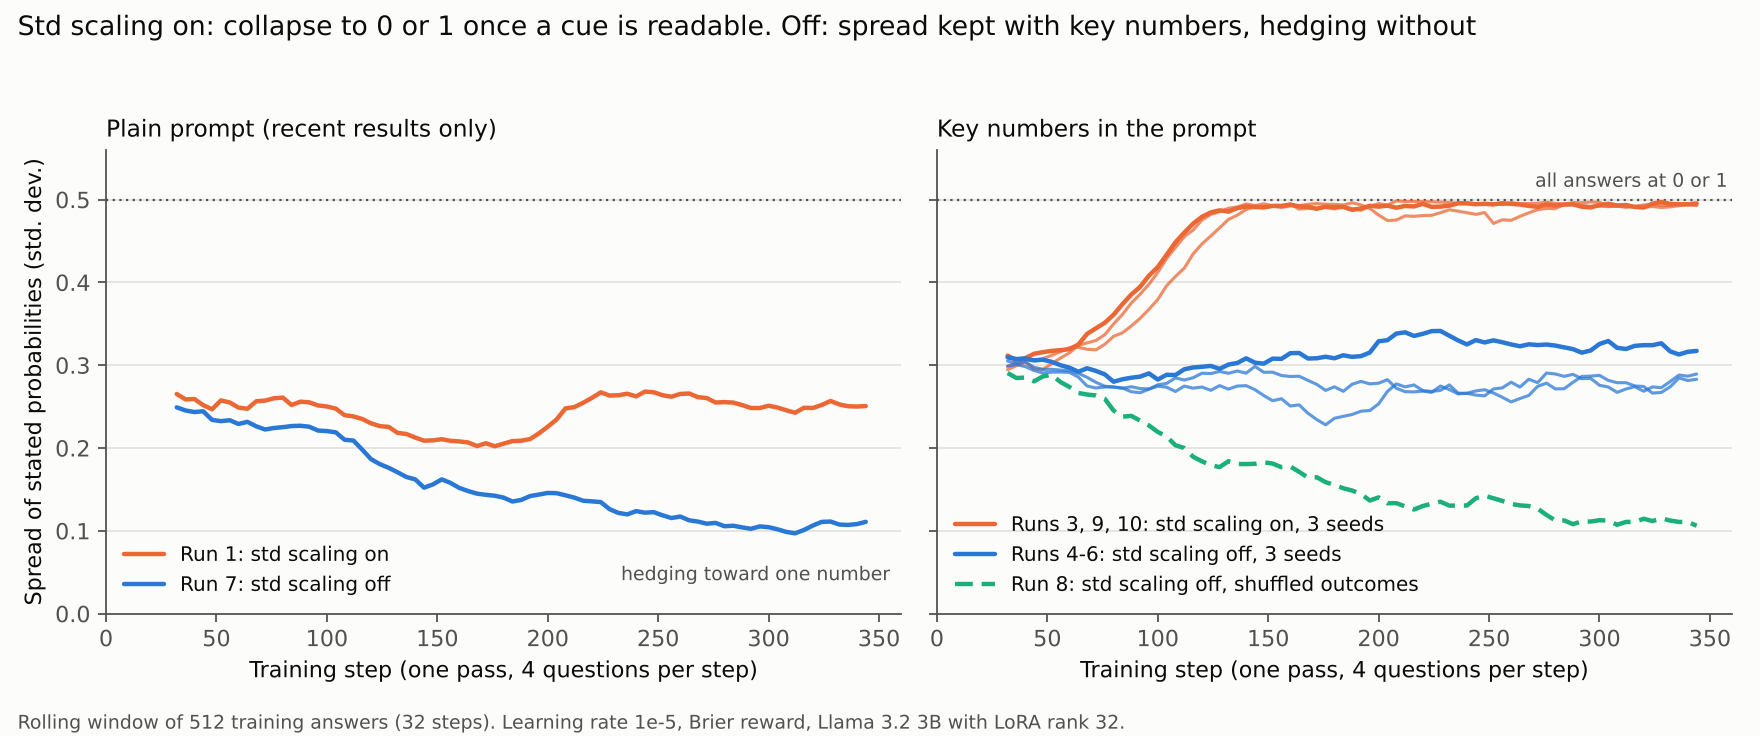
\includegraphics[width=\linewidth]{figures/spread_2x2.png}
\caption{Spread (standard deviation) of stated probabilities during training, over a rolling window of 512 training answers. A model answering only 0 or 1 on balanced questions has spread 0.5; one that hedges toward a single number has spread near 0.}
\label{fig:spread}
\end{figure}

\paragraph{Without the key numbers, one pass of RL changed the average or spread without establishing improved discrimination.}
\begin{itemize}[leftmargin=*]
\item \textbf{Run 1} lowered the average forecast by about 0.06 on both evaluation sets, though not uniformly: on validation, 270 of its 410 forecasts fell and 135 rose. On held-out weather, where one bracket in six resolves YES, its Brier score improved (0.286 to 0.254; $-0.032$, $-0.055$ to $-0.007$). But the untrained model's forecasts shifted down uniformly by the same average amount score better (0.242), and AUC did not improve.
\item \textbf{Run 2}, with twice the training at twice the learning rate, raised AUC from 0.52 to 0.69. But 72\% of its forecasts became near-certain and its Brier score got worse (0.320).
\item \textbf{Run 7}, with std scaling off, contracted its forecasts: all lie between 0.36 and 0.71, around an average of 0.56 (spread 0.17 before training, 0.06 after). That is movement toward a constant, consistent with hedging when the evidence is not used. It does not reach the constant a proper score would prefer for a forecaster without information, since the training yes-rate is 0.491.
\end{itemize}

\par\medskip\noindent\begin{minipage}{\linewidth}
\paragraph{With the key numbers and std scaling off, RL improved the forecasts.} Averaged over three seeds:
\begin{itemize}[leftmargin=*]
\item Brier $-0.031$ ($-0.045$ to $-0.016$);
\item log loss $-0.072$ ($-0.106$ to $-0.036$);
\item AUC $+0.070$ ($+0.036$ to $+0.119$);
\item calibration error $+0.008$ ($-0.024$ to $+0.039$).
\end{itemize}
\end{minipage}\par\medskip
We detect no change in calibration error at this sample size; the interval allows both improvement and deterioration. The seeds barely differ (Brier 0.169 to 0.171, AUC 0.820 to 0.832), and each seed's own interval excludes zero for both Brier and AUC (Table~\ref{tab:boot}). All three seeds improve on core CPI (both measures), year-over-year CPI, the Fed funds rate and unemployment; on payrolls, the noisiest series, there is no consistent improvement: runs 4 and 5 are worse than the untrained model, and run 6 is slightly better (0.269 against 0.273; Appendix~\ref{app:series}, descriptive). The four-answer average flatters the untrained model more than the trained ones, because its four answers disagree more. The average within-question variance is 0.033 for the untrained model and 0.005 to 0.011 for the trained ones. Scored as single answers, the trained models' Brier improvement is larger: 0.177 to 0.182, against 0.233 (Appendix~\ref{app:diag}).

\paragraph{The improvement depends on the real association between inputs and outcomes.} Run 8 repeats run 4, but its training outcomes are permuted once, at random, across all 1,391 training questions and then held fixed. That keeps the yes-rate, breaks the link between each question and its outcome, and leaves 26\% of adjacent threshold pairs within a training ladder inconsistent (none are in the real outcomes). Evaluated on real outcomes, run 8 is \emph{worse} than the untrained model: Brier $+0.035$ ($+0.011$ to $+0.054$), AUC $-0.048$ ($-0.105$ to $-0.008$). Runs 4 to 6 beat it by 0.065 in Brier ($-0.088$ to $-0.039$) and 0.118 in AUC ($+0.077$ to $+0.189$). Its forecasts contract toward one number, as run 7's do: spread 0.074, with 39\% of forecasts between 0.45 and 0.55. Its answers keep their reasoning (median 90 tokens) and are all readable, so the difference from runs 4 to 6 lies in the forecasts, not their format or length. The control shows that the gains need the real outcomes. It does not identify which cues the trained models learned to weigh; we offer cue weighting as an interpretation, not a demonstrated mechanism.

\subsection{With std scaling, RL collapses onto a lookup rule}
\label{sec:collapse}

\begin{table}[t]
\centering\small
\caption{How completely each key-numbers run collapsed (validation econ). The first two columns are shares of single answers; ``exactly the rule's 0/1'' counts answers on the 395 questions with a numeric threshold. ``All 4 identical'' is a share of questions. ``Step'' is the training step at which 90\% of a rolling window of 512 training answers are at or below 0.05 or at or above 0.95 (``near-certain'').}
\label{tab:collapse}
\setlength{\tabcolsep}{4pt}
\begin{tabular}{lccccc}
\toprule
 & Exactly 0 or 1 & Exactly the rule's 0/1 & All 4 identical & Median tokens & Step \\
\midrule
Run 3 (std on, seed 3407) & 99.4\% & 99.9\% & 98.3\% & 7 & 124 \\
Run 9 (std on, seed 1) & 98.8\% & 98.7\% & 94.2\% & 73 & 124 \\
Run 10 (std on, seed 2) & 99.1\% & 94.6\% & 91.7\% & 37 & 136 \\
Runs 4--6 (std off) & 0.0--0.6\% & 0.0--0.6\% & 1.0--6.6\% & 66--74 & never \\
Untrained, key numbers & 4.6\% & 4.2\% & 0.2\% & 110 & -- \\
\bottomrule
\end{tabular}
\end{table}

With GRPO's default scaling, all three key-numbers seeds turn into the same rule (Table~\ref{tab:collapse}). More than 98\% of their answers are exactly 0.00 or 1.00, and almost all of those are the latest-result rule's answer. Averaged over the seeds, they cannot be told apart from the rule: Brier $+0.001$ ($-0.017$ to $+0.020$), AUC $+0.007$ ($-0.008$ to $+0.022$). Against the untrained model with the same prompt, the Brier score does not improve, while log loss and calibration error get much worse (Table~\ref{tab:twobytwo}; calibration error $+0.156$, $+0.045$ to $+0.199$). The std-off seeds beat the std-on seeds on every metric:
\begin{itemize}[leftmargin=*]
\item Brier $-0.048$ ($-0.094$ to $-0.007$);
\item log loss $-0.468$ ($-0.741$ to $-0.236$);
\item calibration error $-0.148$ ($-0.194$ to $-0.027$);
\item AUC $+0.045$ ($+0.021$ to $+0.076$).
\end{itemize}
Their calibration slopes, from regressing the outcomes on the forecasts' log-odds, show the same contrast. The std-on runs have slopes of 0.27 to 0.30, meaning far too extreme forecasts, against 0.80 to 1.07 for runs 4 to 6 (Appendix~\ref{app:diag}).

The collapse happens on the same schedule in every seed, about a third of the way through the pass (Figure~\ref{fig:diagnostics}). Run 10 departs from the rule on 25 threshold questions, 10 of them payrolls. On most of these its four 0/1 answers disagree with each other, so its averaged forecast lands between 0 and 1. Some of those answers follow the count of recent results instead of the latest one. Shrinking answers is not part of the collapse: run 3's answers fell to a median of 7 tokens, but runs 9 and 10 kept short reasoning and still answer 0 or 1.

\paragraph{The collapse is not what the reward asks for.} On the training questions, the latest-result rule is right 84\% of the time when it says YES and wrong 15\% of the time when it says NO. Stated at those hit rates (0.84 and 0.15), it earns a higher average Brier term (0.870) than its 0/1 version (0.847); both exclude the $+0.5$ format bonus that every readable answer gets. The Brier reward therefore prefers the calibrated rule, yet std-scaled GRPO drove all three seeds to the 0/1 version. This is consistent with the mechanism \citet{bereket2025uncalibrated} describe. Dividing each answer's advantage by its group's reward spread inflates small differences between answers that already nearly agree, and with a proper scoring rule that favours confident answers and feeds on itself. We did not run a separate test of the mechanism, such as matching the effective step size without the division.

\begin{figure}[t]
\centering
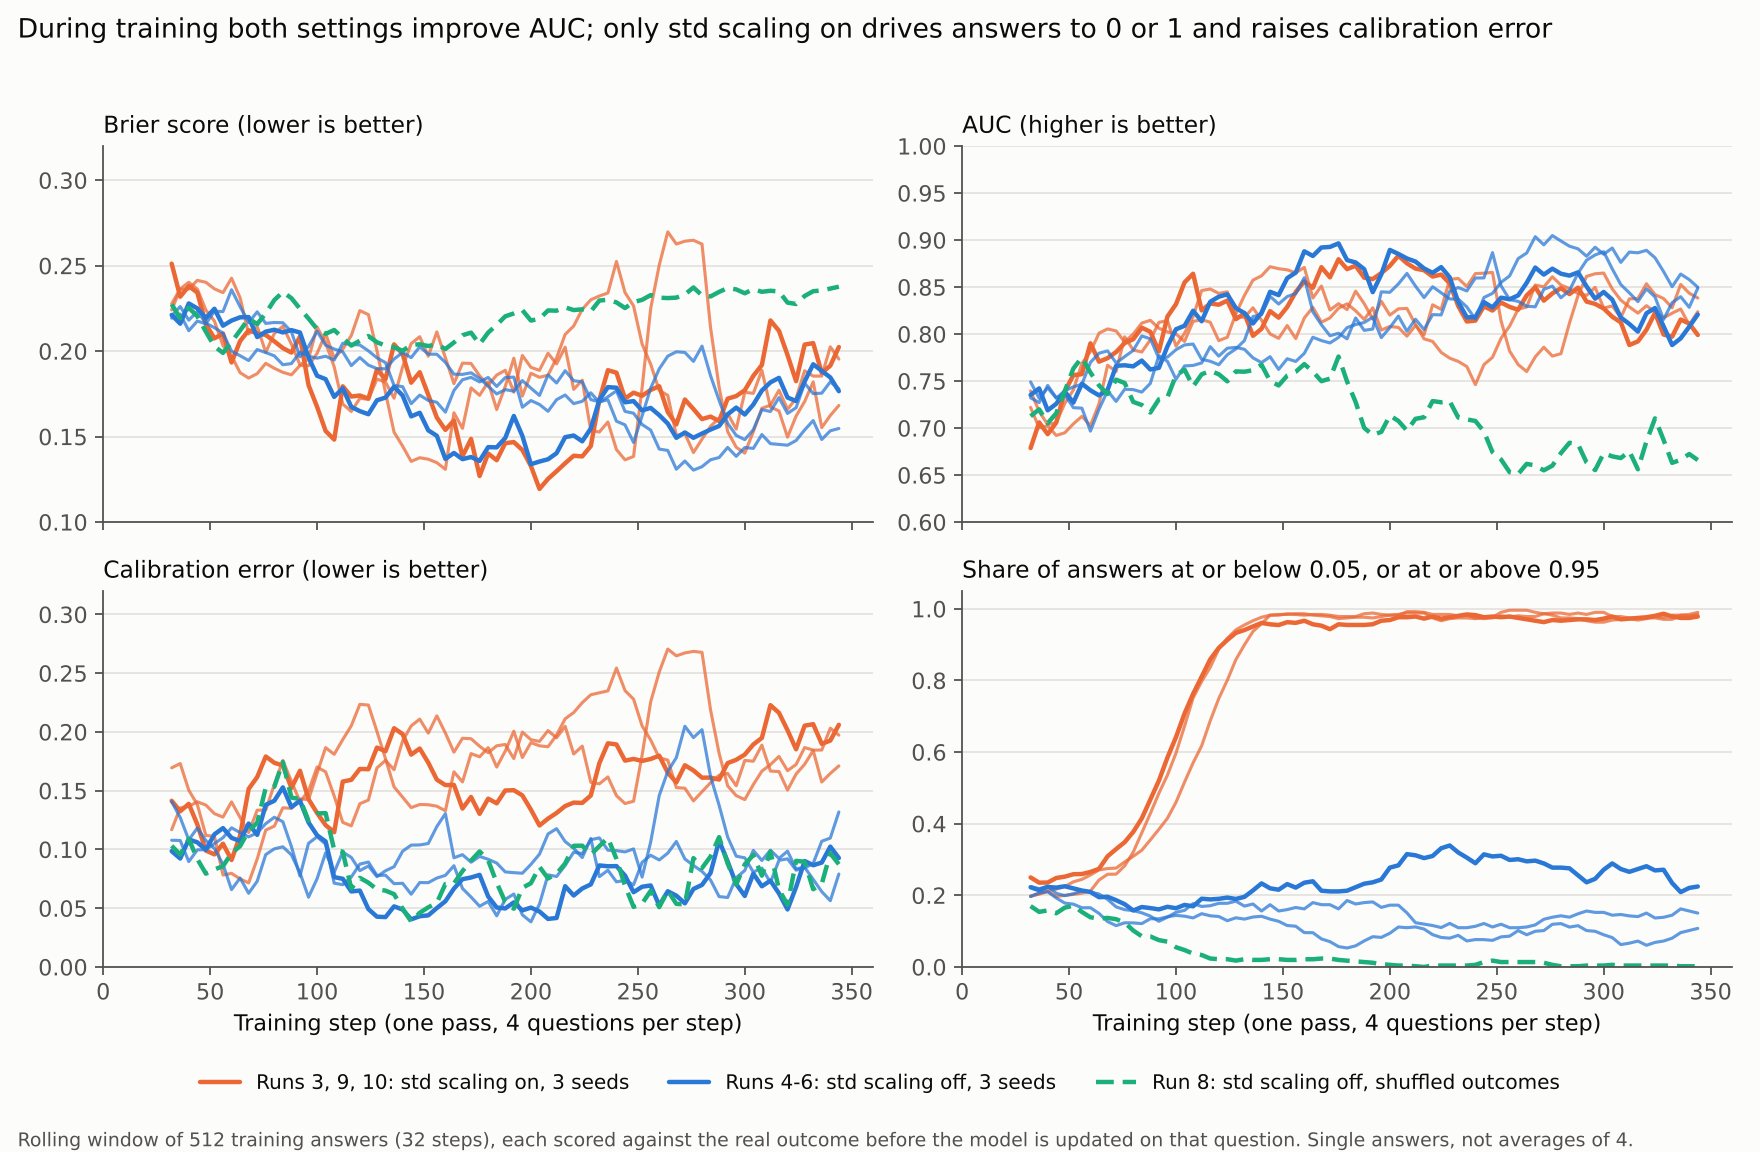
\includegraphics[width=\linewidth]{figures/training_diagnostics.png}
\caption{Key-numbers runs during training: rolling Brier score, AUC, calibration error and share of near-certain answers over 512 training answers, each scored against the real outcome before the model is updated on that question. These curves are descriptive, not clean forward tests: other questions from the same release may already have been rewarded.}
\label{fig:diagnostics}
\end{figure}

\paragraph{During training, both settings learn to rank.} Training-time AUC rises from about 0.72 to 0.80--0.85 with std scaling on or off (Figure~\ref{fig:diagnostics}). What differs is the probabilities. With scaling on, near-certain answers climb from about 20\% to 98\% between steps 75 and 140, and calibration error rises. With it off, answers stay graded. On held-out questions the std-off runs keep their AUC gain (0.82 to 0.83), while the std-on runs sit at the rule's 0.77 to 0.80. Appendix Figure~\ref{fig:hist} shows the end states: two spikes at 0 and 1 for std on, a spread for std off, and one central peak for the shuffled and plain std-off runs.

\subsection{Comparison with simple models}
\label{sec:simple}

\begin{table}[t]
\centering\small
\caption{Runs 4--6 (key numbers, std off; averaged within each draw) against other methods on validation econ. Change = runs 4--6 minus the reference; 95\% intervals resample announcements. Bold: interval excludes 0.}
\label{tab:boot}
\begin{tabular}{lcc}
\toprule
Reference & Brier change & AUC change \\
\midrule
Untrained, key numbers & $\mathbf{-0.031}$ \ci{-0.045}{-0.016} & $\mathbf{+0.070}$ \ci{+0.036}{+0.119} \\
\quad run 4 alone & $\mathbf{-0.033}$ \ci{-0.053}{-0.014} & $\mathbf{+0.071}$ \ci{+0.034}{+0.122} \\
\quad run 5 alone & $\mathbf{-0.030}$ \ci{-0.046}{-0.012} & $\mathbf{+0.063}$ \ci{+0.024}{+0.114} \\
\quad run 6 alone & $\mathbf{-0.030}$ \ci{-0.041}{-0.018} & $\mathbf{+0.075}$ \ci{+0.045}{+0.121} \\
Untrained, best three key-number lines & $-0.019$ \ci{-0.034}{+0.002} & $\mathbf{+0.038}$ \ci{+0.002}{+0.074} \\
Runs 3, 9, 10 (std on) & $\mathbf{-0.048}$ \ci{-0.094}{-0.007} & $\mathbf{+0.045}$ \ci{+0.021}{+0.076} \\
Run 8 (shuffled outcomes) & $\mathbf{-0.065}$ \ci{-0.088}{-0.039} & $\mathbf{+0.118}$ \ci{+0.077}{+0.189} \\
Counting rule & $+0.003$ \ci{-0.026}{+0.040} & $-0.019$ \ci{-0.091}{+0.031} \\
Logistic regression & $+0.008$ \ci{-0.031}{+0.044} & $-0.028$ \ci{-0.057}{+0.011} \\
Gradient-boosted trees, key numbers & $+0.012$ \ci{-0.018}{+0.044} & $\mathbf{-0.033}$ \ci{-0.053}{-0.013} \\
Gradient-boosted trees, key numbers + series & $+0.019$ \ci{-0.006}{+0.049} & $\mathbf{-0.042}$ \ci{-0.069}{-0.018} \\
\bottomrule
\end{tabular}
\end{table}

Table~\ref{tab:boot} compares the trained models with every reference on the same questions.
\begin{itemize}[leftmargin=*]
\item \textbf{Logistic regression.} The trained models score Brier 0.170 and AUC 0.827, against 0.163 and 0.855. The paired intervals include zero, so this sample does not resolve the difference; it establishes neither equivalence nor an advantage for RL. The same holds against the counting rule (0.168 and 0.846).
\item \textbf{Gradient-boosted trees.} The trees are a stronger simple reference on the supplied features: the trained models trail them in AUC by 0.033 and 0.042, with both intervals excluding zero. On the test split the gap is smaller (0.013 and 0.017) and its intervals include zero (\S\ref{sec:test}).
\item \textbf{The best untrained prompt.} Against the three-line prompt from the ablation, the trained models' AUC is higher by 0.038 (+0.002 to +0.074), but the Brier difference is not resolved.
\item \textbf{Skill relative to the base rate.} RL takes the untrained model from 0.17 to about 0.30; the logistic regression reaches 0.33, the trees 0.38 and the market 0.75 (Appendix~\ref{app:skill}).
\end{itemize}
The market prices information that is not in our prompt, such as consensus forecasts and nowcasts. It is an external benchmark with a broader information set, and nothing here suggests the model is economically competitive with it.

\subsection{Weather}
\label{sec:weather}

We find no useful discrimination on the evaluated weather brackets under this evidence setup, except from the market. Every rule built from recent highs has AUC below 0.5, and the base rate (Brier 0.139) beats every model and rule. RL does not change this. The std-off runs average 0.216, against 0.223 for the untrained model with the same prompt ($-0.007$, $-0.019$ to $+0.007$). The std-on runs are worse: 0.283, or $+0.060$ ($+0.038$ to $+0.080$), because they carry their 0/1 answers over. These intervals resample days.

\subsection{Test set}
\label{sec:test}

After all development, eleven models were scored once on the test split: the untrained model with each prompt, and runs 1 and 3 to 10 (run 2, optional in the plan, was not scored). The split has 479 priced questions from 36 releases and 13 announcements, June to October 2026 (yes-rate 0.409). The model comparisons, the rules for reading them and the code that applies those rules were committed to the repository before any language model was scored on the test split (\texttt{eval/test\_plan.md}). No model was retrained. Each run's saved adapter was loaded unchanged, and before any test question every model re-answered 80 validation questions and reproduced its stored answers (83\% to 100\% of them word for word). The test questions were not entirely unseen: dry runs of the evaluation code, with made-up model answers, computed the baselines on them, starting before the plan's first commit. No language model was scored on them before the final run; Appendix~\ref{app:timeline} gives the timeline. We fixed three predictions:
\begin{itemize}[leftmargin=*]
\item \textbf{P1:} runs 4--6 improve on the untrained model with the same prompt, in Brier score and, as a separate conclusion, in AUC.
\item \textbf{P2:} runs 4--6 beat runs 3, 9 and 10 in both log loss and calibration error.
\item \textbf{P3:} runs 3, 9 and 10 each again give at least 90\% of answers exactly 0 or 1, and at least 90\% exactly the latest-result rule's 0 or 1.
\end{itemize}
P1 and P2 hold if their intervals exclude 0 in the predicted direction; the right direction with an interval including 0 would have been ``consistent but not confirmed''. P3 holds if each of the three std-on runs meets both 90\% thresholds.

\begin{table}[t]
\centering\small
\caption{The predictions fixed before the language models were scored on test, with selected secondary comparisons, on validation and test. KN = key-numbers prompt. Change = compared models minus reference, with groups of seeds averaged within each draw; 95\% intervals resample announcements (13 in each split). Bold: interval excludes 0. Secondary comparisons are descriptive; all of them are in the repository's \texttt{eval/test\_results.md}.}
\label{tab:test}
\setlength{\tabcolsep}{3.5pt}
\resizebox{\linewidth}{!}{%
\begin{tabular}{lllccc}
\toprule
 & Comparison & Metric & Validation & Test & Reading \\
\midrule
P1 & Runs 4--6 vs untrained, KN & Brier & $\mathbf{-0.031}$ {\scriptsize[$-0.045$, $-0.016$]} & $\mathbf{-0.025}$ {\scriptsize[$-0.034$, $-0.016$]} & holds \\
 &  & AUC & $\mathbf{+0.070}$ {\scriptsize[$+0.036$, $+0.119$]} & $\mathbf{+0.033}$ {\scriptsize[$+0.018$, $+0.054$]} & holds \\
P2 & Runs 4--6 vs runs 3, 9, 10 & Log loss & $\mathbf{-0.468}$ {\scriptsize[$-0.741$, $-0.236$]} & $\mathbf{-0.409}$ {\scriptsize[$-0.676$, $-0.195$]} & \multirow{2}{*}{holds} \\
 &  & Calibration error & $\mathbf{-0.148}$ {\scriptsize[$-0.194$, $-0.027$]} & $\mathbf{-0.109}$ {\scriptsize[$-0.134$, $-0.004$]} &  \\
P3 & Runs 3, 9, 10 & Answers exactly 0 or 1 & 98.8--99.4\% & 99.3--99.8\% & \multirow{2}{*}{holds} \\
 &  & Answers exactly the rule's & 94.6--99.9\% & 95.1--99.8\% &  \\
\midrule
S1 & Runs 4--6 vs logistic regression & Brier & $+0.008$ {\scriptsize[$-0.031$, $+0.044$]} & $+0.010$ {\scriptsize[$-0.014$, $+0.029$]} &  \\
 &  & AUC & $-0.028$ {\scriptsize[$-0.057$, $+0.011$]} & $-0.011$ {\scriptsize[$-0.035$, $+0.016$]} &  \\
S8 & Runs 4--6 vs trees, KN & AUC & $\mathbf{-0.033}$ {\scriptsize[$-0.053$, $-0.013$]} & $-0.013$ {\scriptsize[$-0.039$, $+0.017$]} &  \\
 & Runs 4--6 vs trees, KN + series & AUC & $\mathbf{-0.042}$ {\scriptsize[$-0.069$, $-0.018$]} & $-0.017$ {\scriptsize[$-0.039$, $+0.005$]} &  \\
S2 & Untrained: KN vs plain prompt & AUC & $\mathbf{+0.237}$ {\scriptsize[$+0.189$, $+0.312$]} & $\mathbf{+0.248}$ {\scriptsize[$+0.148$, $+0.367$]} &  \\
S3 & Runs 3, 9, 10 vs untrained, KN & Log loss & $\mathbf{+0.396}$ {\scriptsize[$+0.142$, $+0.690$]} & $\mathbf{+0.343}$ {\scriptsize[$+0.113$, $+0.629$]} &  \\
 &  & AUC & $+0.025$ {\scriptsize[$-0.029$, $+0.088$]} & $\mathbf{-0.037}$ {\scriptsize[$-0.075$, $-0.006$]} &  \\
S5 & Run 1 vs untrained, plain & Brier & $-0.005$ {\scriptsize[$-0.024$, $+0.017$]} & $\mathbf{-0.022}$ {\scriptsize[$-0.045$, $-0.003$]} &  \\
S6 & Run 8 vs untrained, KN & Brier & $\mathbf{+0.035}$ {\scriptsize[$+0.011$, $+0.054$]} & $\mathbf{+0.061}$ {\scriptsize[$+0.046$, $+0.075$]} &  \\
S7 & Runs 4--6 vs run 8 & AUC & $\mathbf{+0.118}$ {\scriptsize[$+0.077$, $+0.189$]} & $\mathbf{+0.061}$ {\scriptsize[$+0.035$, $+0.098$]} &  \\
\bottomrule
\end{tabular}}
\end{table}

\begin{table}[t]
\centering\small
\caption{Test scores (479 priced questions, 13 announcements; yes-rate 0.409). Four-answer averages; for the groups of three seeds, the average and the range across seeds. Every method is in Appendix Table~\ref{tab:testmain}.}
\label{tab:testscores}
\setlength{\tabcolsep}{4pt}
\begin{tabular}{lcccc}
\toprule
Method & Brier $\downarrow$ & Log loss $\downarrow$ & ECE $\downarrow$ & AUC $\uparrow$ \\
\midrule
Market price (never shown to the model) & 0.073 & 0.236 & 0.038 & 0.967 \\
Gradient-boosted trees, key numbers + series & 0.125 & 0.384 & 0.064 & 0.906 \\
Logistic regression, key numbers & 0.130 & 0.400 & 0.057 & 0.899 \\
Counting rule & 0.138 & 0.461 & 0.059 & 0.880 \\
Latest-result rule (0/1) & 0.193 & 0.889 & 0.188 & 0.804 \\
\midrule
Untrained, key numbers & 0.165 & 0.503 & 0.110 & 0.855 \\
Runs 4, 5, 6: key numbers, std off & 0.139 {\scriptsize[.135, .146]} & 0.437 {\scriptsize[.42, .46]} & 0.076 {\scriptsize[.05, .09]} & 0.888 {\scriptsize[.886, .892]} \\
Runs 3, 9, 10: key numbers, std on & 0.187 {\scriptsize[.177, .194]} & 0.846 {\scriptsize[.78, .90]} & 0.185 {\scriptsize[.17, .19]} & 0.818 {\scriptsize[.80, .84]} \\
Run 8: key numbers, std off, shuffled outcomes & 0.226 & 0.645 & 0.176 & 0.828 \\
\bottomrule
\end{tabular}
\end{table}

\paragraph{All three predictions hold.} Table~\ref{tab:test} gives them next to their validation values; resampling single releases instead of announcements gives the same readings. P1's Brier gain ($-0.025$) is close to its validation size, and each seed's own interval excludes zero for both Brier and AUC (Table~\ref{tab:seedtest}). The AUC gain ($+0.033$) is about half its validation size. P2's calibration-error interval only just excludes zero. The std-on models' test answers are as collapsed as their validation answers: 99.3\% to 99.8\% are exactly 0 or 1, and 95.1\% to 99.8\% exactly the rule's 0 or 1, with run 10 again departing most.

\paragraph{Secondary comparisons.} As on validation, the trained models do not outperform the logistic regression or the trees (Table~\ref{tab:testscores}). Runs 4--6 score Brier 0.139 and AUC 0.888, against 0.130 and 0.899 for the logistic regression and 0.125 and 0.906 for the trees with the series. The simple models are numerically ahead on every metric, but no Brier or AUC difference from them is resolved on test. The AUC gap to the trees, which excluded zero on validation, is smaller here. Shuffled outcomes again make the model worse, and the key-numbers block again does most of the work: it raises the untrained model's AUC by 0.248. Two secondary results differ from validation. The std-on runs now have lower AUC than the untrained model, which fits the collapse: on test the untrained model ranks the questions better than the rule those runs copy (AUC 0.855 against 0.804), while on validation it ranked them worse. And run 1 improves its Brier score. It again lowers its average forecast by about 0.06, and a uniform shift of the untrained model's forecasts by the same amount reproduces 0.016 of its 0.022 gain (exploratory). These are two of 36 secondary intervals, with no correction for multiple comparisons.

\paragraph{Methods that read the recent results scored better on test.} Every such method has a lower Brier score and a higher AUC than on validation; calibration error does not always improve (the untrained key-numbers model's rises from 0.060 to 0.110). The untrained key-numbers model's AUC rises from 0.757 to 0.855, the logistic regression's from 0.855 to 0.899, and runs 4--6 reach 0.886 to 0.892 (Brier 0.135 to 0.146). The market and the base rate score slightly worse. These comparisons describe the period; they do not show why it differed. Exploratory: runs 4--6 forecast YES too often for the test period (average forecast 0.44 to 0.50 against a yes-rate of 0.409), and their calibration slopes rise above 1 (1.19 to 1.51), so their forecasts are not extreme enough. Appendix~\ref{app:test} has every method's test scores, diagnostics, per-series results and a reliability diagram.

\section{Discussion}

\paragraph{What RL did here.} With the evidence spelled out and std scaling off, RL improved the forecasts from the supplied evidence under our training setup. Forecasts became better ordered, calibration error did not detectably change, and the gains depended on real outcomes. We find no predictive advantage over simple models trained on these features: the trained models do not outperform a logistic regression or the counting rule, and they trail gradient-boosted trees: clearly in validation AUC, and only in direction on test. The expected proper score is maximized by the conditional probability of the event given the information used. When a model's answers do not depend on the evidence, the best it can do is a constant. That is the direction RL took with the plain prompt (run 7) and with shuffled outcomes (run 8): toward a constant, though finite training does not guarantee reaching it. These patterns held on the test split, scored once. In our runs, one pass of RL improved the use of evidence the model could already read. Only with twice the training at twice the learning rate (run 2) did it learn some ordering from the plain prompt, and then at the cost of calibration.

\paragraph{Practical lessons.}
\begin{itemize}[leftmargin=*]
\item \textbf{Check GRPO's std scaling when the reward is a proper score.} In our three-seed comparison, the default produced a collapse that a Brier score alone would not reveal: the collapsed runs' training Brier score improved. This agrees with \citet{bereket2025uncalibrated} and with the recent forecasting papers that drop the scaling \citep{turtel2026proper,ye2026alphabet}. We do not show that disabling it is enough for calibrated forecasting in other settings.
\item \textbf{Compare trained models with rules built from their own prompts.} The collapse was obvious only next to the latest-result rule, and the limits of the gains only next to the logistic regression and the trees.
\item \textbf{Report AUC and a shift-matched baseline next to the Brier score.} A uniform shift of the untrained model's forecasts to run 1's average reproduces, and exceeds, run 1's weather gain.
\end{itemize}

\paragraph{Limitations.}
\begin{itemize}[leftmargin=*]
\item \textbf{Scope.} We study one model size and family (the \texttt{unsloth/Llama-3.2-3B-Instruct} 16-bit checkpoint; the exact revision was not pinned), LoRA training for one pass at one learning rate, and one domain: scheduled numeric releases forecast a day ahead. Only the key-numbers conditions have three seeds. We did not compare with supervised fine-tuning on the same questions or with RL from the best three-line prompt, which a claim of an advantage specific to RL, or of an optimal prompt, would need.
\item \textbf{Sample size.} Validation and test each contain 13 announcement clusters. Intervals account for dependence within announcements but may not capture dependence across time, so they are rough, and per-series results are descriptive. Settings were chosen on validation, which is why the final numbers come from a test split scored once. The test split is itself one five-month period, in which methods that read the recent results scored better than on validation.
\item \textbf{The key-numbers block is hand-designed for threshold questions.} The general lesson is that evidence must be legible to the model, not that this block suits other questions.
\item \textbf{Pooled AUC} compares questions across thresholds and series, so part of it reflects ordering the thresholds within a release coherently. It should not be read as general skill at predicting the next economic value. The trained models still order 28\% to 35\% of adjacent threshold pairs the wrong way (Appendix~\ref{app:diag}).
\item \textbf{Training-time curves are not clean forward tests.} Questions from the same release can be rewarded before others are answered.
\item \textbf{Context order.} During the late-2025 U.S.\ government shutdown, delayed releases put one pair of months out of calendar order in the context of 50 validation questions. Both values were public; prompts were left unchanged so every run sees identical inputs.
\item \textbf{The market is a benchmark, not ground truth.} Low-priced contracts are biased \citep{burgi2026makers}.
\end{itemize}

\section{Conclusion}

In this controlled setting, how the evidence is presented and how advantages are normalized decide whether Brier-reward GRPO improves a small language model's forecasts:
\begin{itemize}[leftmargin=*]
\item With the evidence in raw form, one pass of RL lowered the average forecast (std scaling on) or contracted the forecasts toward a constant (std off).
\item With the comparisons spelled out, GRPO's default std scaling turned the model into a 0/1 lookup rule in every seed.
\item Without that scaling, RL improved both the Brier score and discrimination, without establishing an advantage over simple supervised models on the same features.
\end{itemize}
The last two held on a later test split, scored once against precommitted model comparisons.
We hope the controls used here become standard in RL-for-forecasting work: rules built from the prompt, shuffled outcomes, shift-matched baselines, multiple seeds, announcement-level intervals, and AUC next to the Brier score.

\bibliographystyle{plainnat}
\bibliography{refs}

\clearpage
\appendix

\section{Prompt}
\label{app:prompt}

\paragraph{System prompt.}
\begin{quote}\small
You are a careful forecaster. You will get a yes/no question about an upcoming data release or measurement, the current date, and sometimes recent results for the same data series. Think it through briefly (under 150 words), then end with one final line in exactly this form: Probability: 0.XX where 0.XX is your probability, between 0 and 1, that the question resolves YES.
\end{quote}

\paragraph{User message (a training question, key-numbers prompt).} The plain prompt is the same without the key-numbers block. The question's date is also passed to Llama's chat template.
\begin{quote}\footnotesize\ttfamily\raggedright
Current date: Tuesday, June 11, 2024, 8:25 AM Eastern\\[3pt]
Question: If the Consumer Price Index (CPI) increases by more than 0.1\% in May 2024, then the market resolves to Yes.\\[3pt]
Recent results in this series (oldest first; all were public before this question):\\
- CPI in Nov 2023: 0.1\\
- CPI in Dec 2023: 0.3\\
- CPI in Jan 2024: 0.3\\
- CPI in Feb 2024: 0.4\\
- CPI in Mar 2024: 0.4\\
- CPI in Apr 2024: 0.3\\[3pt]
Key numbers (worked out from the question and the recent results above):\\
- This question resolves YES if the result is above 0.1\%.\\
- Latest result (CPI in Apr 2024): 0.3\%, 0.2 percentage points above the threshold.\\
- Change from the result before: -0.1 percentage points (from 0.4\% to 0.3\%).\\
- Recent results that would have resolved YES: 5 of 6.\\
- Recent results: average 0.3\%, lowest 0.1\%, highest 0.4\%.\\[3pt]
What is the probability that this question resolves YES?
\end{quote}
This question resolved NO (May 2024 CPI was flat); the market priced YES at 0.28.

\section{Training and evaluation settings}
\label{app:hyper}

\begin{table}[H]
\centering\small
\begin{tabularx}{\linewidth}{lX}
\toprule
Base model & \texttt{unsloth/Llama-3.2-3B-Instruct} (16-bit), Unsloth 2026.10, TRL 0.22.2, vLLM 0.11.2 \\
LoRA & rank 32, $\alpha$ 32, q/k/v/o and gate/up/down projections; 48.6M trainable parameters (1.49\%) \\
GRPO & 4 answers per question, 4 questions per step (16 answers), 347 steps (one pass) \\
Loss & TRL default (\texttt{dapo}), no KL penalty ($\beta=0$), gradient clipping at 1.0 \\
Optimiser & AdamW 8-bit, learning rate $10^{-5}$, cosine decay, 10\% warm-up, weight decay 0.001 \\
Sampling in training & up to 256 new tokens \\
Rewards & readable: $1-(p-y)^2 + 0.5$; unreadable: $-1$ \\
Evaluation sampling & 4 answers, temperature 0.7, top-$p$ 0.95, up to 320 tokens, seed 3407 \\
Hardware & one NVIDIA T4 (16\,GB), Kaggle free tier; 1.3 to 2.7 hours per training run \\
\bottomrule
\end{tabularx}
\end{table}

Total compute: about 18 GPU-hours of training, 5 of evaluation and the prompt ablation, and 4 of setup and baselines, about 27 GPU-hours before the test split; scoring it took about 3.5 more (a 40-minute run of the loading check alone, then the scored run of about 2.8 hours), about 30 in total.

\section{Baseline definitions}
\label{app:baselines}

The five key-number features are computed from the question's threshold and the six recent results $v_1,\dots,v_6$ (oldest first):
\begin{enumerate}[leftmargin=*]
\item the share of recent results that would have resolved YES;
\item whether the latest result would have (0 or 1);
\item the latest result's signed distance from the YES region, divided by the series' typical move;
\item the same distance for the recent average;
\item the change in that distance from the previous result to the latest.
\end{enumerate}
The ``typical move'' is the median absolute change between consecutive recent results. When that is 0, we use the mean absolute change, and for a flat series 5\% of the threshold. The scaled distances are clipped to $\pm 5$.

The logistic regression is fitted by Newton's method with an L2 penalty of 1 (not on the intercept). The gradient-boosted trees use scikit-learn's histogram gradient boosting, with at least 20 questions per leaf, L2 regularization 1 and no early stopping. Their settings were chosen from eight combinations (depth 2 or 3, learning rate 0.03 or 0.1, 100 or 300 trees) by 5-fold cross-validation on the training questions, with each announcement kept in one fold and the lowest log loss winning. Both versions chose depth 3, learning rate 0.03 and 100 trees. Fed-decision questions, which have no numeric threshold, get the series' training yes-rate under every rule-based baseline.

\section{Additional diagnostics (validation econ)}
\label{app:diag}

\begin{table}[H]
\centering\small
\caption{Diagnostics from the saved answers. ``Single answers'' is the mean Brier score of the individual answers, with an unreadable answer counted as 0.5. Its gap to the Brier score of the four-answer average computed the same way (unreadable answers as 0.5) is the average within-question variance of the four answers. The four-answer column uses the primary rule (the average of readable answers), which differs from that by at most 0.002. Ladder violations are among 362 adjacent threshold pairs. Calibration slope and intercept come from a logistic regression of the outcome on the forecast's log-odds, with forecasts clipped to $[0.01, 0.99]$ first; a slope of 1 is ideal, and below 1 means forecasts too extreme. ``Equal weight'' averages each announcement's Brier score.}
\setlength{\tabcolsep}{6pt}
\resizebox{\linewidth}{!}{%
\begin{tabular}{lcccccc}
\toprule
 & \shortstack{Brier\\(4-answer)} & \shortstack{Brier\\(single answers)} & \shortstack{Ladder\\violations} & Slope & Intercept & \shortstack{Brier\\(equal weight)} \\
\midrule
Untrained, plain & 0.272 & 0.304 & 48\% & 0.13 & $-0.17$ & 0.285 \\
Untrained, key numbers & 0.201 & 0.233 & 38\% & 0.82 & $-0.11$ & 0.211 \\
Untrained, three lines & 0.190 & 0.225 & 38\% & 0.70 & 0.00 & 0.193 \\
Runs 4--6 (std off) & 0.169--0.171 & 0.177--0.182 & 28--35\% & 0.80--1.07 & $-0.42$ to $-0.07$ & 0.174--0.181 \\
Runs 3, 9, 10 (std on) & 0.211--0.223 & 0.224--0.230 & 0--2\% & 0.27--0.30 & $-0.16$ to 0.02 & 0.221--0.226 \\
Run 8 (shuffled) & 0.236 & 0.240 & 41\% & 2.44 & $-0.56$ & 0.242 \\
Logistic regression & 0.163 & -- & 6\% & 0.61 & 0.21 & 0.162 \\
Trees, key numbers + series & 0.151 & -- & 2\% & 0.86 & 0.35 & 0.149 \\
Counting rule & 0.168 & -- & 0\% & 0.48 & $-0.16$ & 0.160 \\
\bottomrule
\end{tabular}}
\end{table}

Resampling single releases (36) instead of announcements (13) gives very similar intervals for every comparison in Tables~\ref{tab:twobytwo} and~\ref{tab:boot}, and the main conclusions are unchanged. Two readings change. Run 8's AUC change against the untrained model becomes unresolved ($-0.048$, $-0.100$ to $+0.003$), while its Brier deterioration and the main setup's advantage over run 8 still exclude zero. And runs 4--6's Brier change against the best three-line prompt becomes resolved ($-0.019$, $-0.036$ to $-0.001$). Both versions are in the repository's \texttt{eval/analysis} folder.

\begin{figure}[H]
\centering
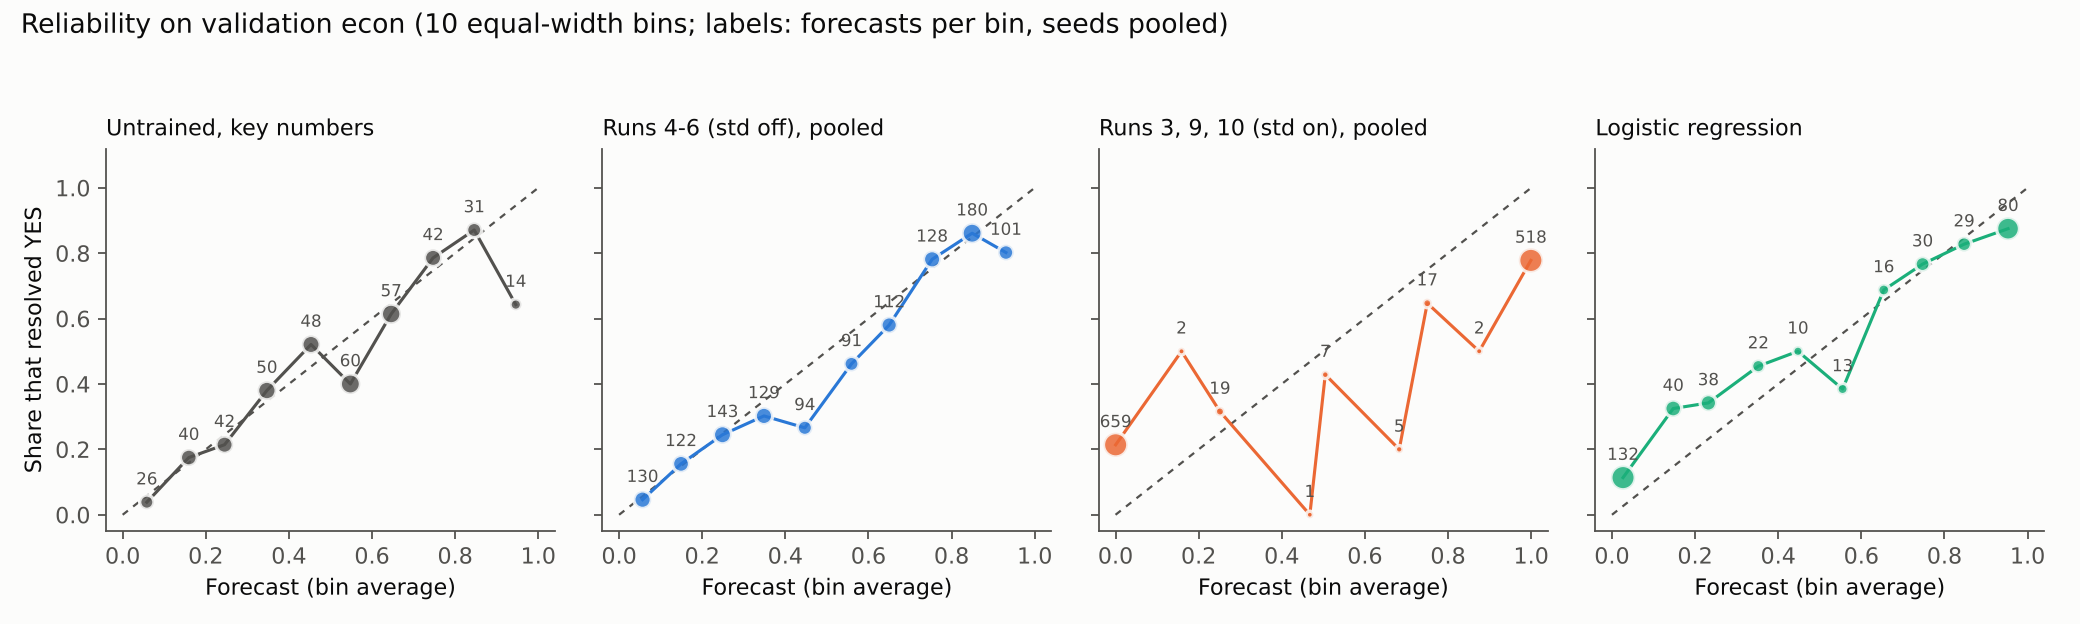
\includegraphics[width=\linewidth]{figures/reliability_validation.png}
\caption{Reliability diagrams on validation econ, 10 equal-width bins, with the number of forecasts in each bin (three seeds pooled where noted). The std-on runs put almost every forecast at 0 or 1.}
\label{fig:reliability}
\end{figure}

\section{Per-series results}
\label{app:series}

\begin{table}[H]
\centering\small
\caption{Brier score by series, validation econ (3 to 5 releases each, so descriptive only).}
\begin{tabular}{lccccccc}
\toprule
Series & $n$ & Untrained KN & Run 4 & Run 5 & Run 6 & Logistic & Latest-result rule \\
\midrule
Core CPI, month & 42 & 0.146 & 0.088 & 0.077 & 0.077 & 0.071 & 0.095 \\
Core CPI, year & 76 & 0.201 & 0.134 & 0.153 & 0.175 & 0.115 & 0.145 \\
CPI, month & 45 & 0.167 & 0.198 & 0.162 & 0.156 & 0.209 & 0.267 \\
CPI, year & 75 & 0.218 & 0.184 & 0.185 & 0.178 & 0.176 & 0.227 \\
Fed funds rate & 33 & 0.146 & 0.065 & 0.071 & 0.091 & 0.032 & 0.000 \\
Unemployment & 50 & 0.134 & 0.077 & 0.093 & 0.110 & 0.049 & 0.060 \\
Payrolls & 74 & 0.273 & 0.291 & 0.300 & 0.269 & 0.359 & 0.541 \\
Fed decision (no threshold) & 15 & 0.368 & 0.342 & 0.335 & 0.330 & 0.160 & 0.160 \\
\bottomrule
\end{tabular}
\end{table}

\section{Test split details}
\label{app:test}

The language models were scored once on test, after the comparisons in Table~\ref{tab:test} were committed; the baselines' test scores had been computed earlier (Appendix~\ref{app:timeline}). Everything in this appendix is descriptive; the calibration slopes, per-series results and reliability diagram were computed after scoring.

\begin{table}[H]
\centering\small
\caption{Each seed of runs 4--6 against the untrained model with the key-numbers prompt (P1 for single runs). 95\% intervals resample announcements. All intervals exclude 0.}
\label{tab:seedtest}
\setlength{\tabcolsep}{3.5pt}
\begin{tabular}{lcccc}
\toprule
 & \multicolumn{2}{c}{Validation} & \multicolumn{2}{c}{Test} \\
\cmidrule(lr){2-3}\cmidrule(lr){4-5}
 & Brier change & AUC change & Brier change & AUC change \\
\midrule
Run 4 & $-0.033$ \ci{-0.053}{-0.014} & $+0.071$ \ci{+0.034}{+0.122} & $-0.030$ \ci{-0.041}{-0.019} & $+0.031$ \ci{+0.013}{+0.053} \\
Run 5 & $-0.030$ \ci{-0.046}{-0.012} & $+0.063$ \ci{+0.024}{+0.114} & $-0.027$ \ci{-0.039}{-0.014} & $+0.037$ \ci{+0.023}{+0.057} \\
Run 6 & $-0.030$ \ci{-0.041}{-0.018} & $+0.075$ \ci{+0.045}{+0.121} & $-0.018$ \ci{-0.028}{-0.008} & $+0.033$ \ci{+0.012}{+0.057} \\
\bottomrule
\end{tabular}
\end{table}

\begin{table}[H]
\centering\small
\caption{Every method on the 479 priced test econ questions (36 releases, 13 announcements; yes-rate 0.409). Four-answer averages; for the two groups of three seeds, the average and the range across seeds. Bold: best short of the market.}
\label{tab:testmain}
\setlength{\tabcolsep}{4pt}
\begin{tabular}{lcccc}
\toprule
Method & Brier $\downarrow$ & Log loss $\downarrow$ & ECE $\downarrow$ & AUC $\uparrow$ \\
\midrule
Market price (never shown to the model) & 0.073 & 0.236 & 0.038 & 0.967 \\
\midrule
Gradient-boosted trees, key numbers + series & \textbf{0.125} & \textbf{0.384} & 0.064 & \textbf{0.906} \\
Gradient-boosted trees, key numbers & 0.127 & 0.393 & 0.046 & 0.901 \\
Logistic regression, key numbers & 0.130 & 0.400 & 0.057 & 0.899 \\
Counting rule & 0.138 & 0.461 & 0.059 & 0.880 \\
Latest-result rule (0/1) & 0.193 & 0.889 & 0.188 & 0.804 \\
Base rate & 0.247 & 0.687 & 0.085 & 0.554 \\
Always 0.5 & 0.250 & 0.693 & 0.091 & 0.500 \\
\midrule
Untrained, plain prompt & 0.265 & 0.732 & 0.168 & 0.607 \\
Run 1: plain, std on & 0.243 & 0.679 & 0.132 & 0.627 \\
Run 7: plain, std off & 0.265 & 0.724 & 0.174 & 0.594 \\
\midrule
Untrained, key numbers & 0.165 & 0.503 & 0.110 & 0.855 \\
Runs 3, 9, 10: key numbers, std on & 0.187 {\scriptsize[.177, .194]} & 0.846 {\scriptsize[.78, .90]} & 0.185 {\scriptsize[.17, .19]} & 0.818 {\scriptsize[.80, .84]} \\
Runs 4, 5, 6: key numbers, std off & 0.139 {\scriptsize[.135, .146]} & 0.437 {\scriptsize[.42, .46]} & 0.076 {\scriptsize[.05, .09]} & 0.888 {\scriptsize[.886, .892]} \\
Run 8: key numbers, std off, shuffled outcomes & 0.226 & 0.645 & 0.176 & 0.828 \\
\bottomrule
\end{tabular}
\end{table}

\begin{table}[H]
\centering\small
\caption{Diagnostics on test econ, defined as in Appendix~\ref{app:diag}. Ladder violations are among 431 adjacent threshold pairs. Every trained run's answers were at least 99.95\% readable, the untrained models' 96.8\% (key numbers) and 98.8\% (plain); counting unreadable answers as 0.5 changes no Brier score by more than 0.002.}
\setlength{\tabcolsep}{6pt}
\resizebox{\linewidth}{!}{%
\begin{tabular}{lcccccc}
\toprule
 & \shortstack{Brier\\(4-answer)} & \shortstack{Brier\\(single answers)} & \shortstack{Ladder\\violations} & Slope & Intercept & \shortstack{Brier\\(equal weight)} \\
\midrule
Untrained, plain & 0.265 & 0.297 & 49\% & 0.53 & $-0.55$ & 0.275 \\
Untrained, key numbers & 0.165 & 0.196 & 40\% & 1.56 & $-0.56$ & 0.167 \\
Runs 4--6 (std off) & 0.135--0.146 & 0.143--0.157 & 33--36\% & 1.19--1.51 & $-0.66$ to $-0.21$ & 0.134--0.151 \\
Runs 3, 9, 10 (std on) & 0.177--0.194 & 0.193--0.195 & 0--2\% & 0.31--0.36 & $-0.52$ to $-0.29$ & 0.179--0.193 \\
Run 8 (shuffled) & 0.226 & 0.230 & 41\% & 5.73 & $-1.48$ & 0.226 \\
Logistic regression & 0.130 & -- & 4\% & 0.89 & 0.03 & 0.132 \\
Trees, key numbers + series & 0.125 & -- & 1\% & 1.09 & 0.01 & 0.127 \\
Counting rule & 0.138 & -- & 0\% & 0.63 & $-0.13$ & 0.136 \\
Market & 0.073 & -- & 4\% & 0.90 & $-0.22$ & 0.080 \\
\bottomrule
\end{tabular}}
\end{table}

\begin{table}[H]
\centering\small
\caption{Brier score by series, test econ (3 to 5 releases each, so descriptive only).}
\setlength{\tabcolsep}{4pt}
\begin{tabular}{lcccccccc}
\toprule
Series & $n$ & Untrained KN & Run 4 & Run 5 & Run 6 & Logistic & Latest-result rule & Market \\
\midrule
Core CPI, month & 52 & 0.127 & 0.086 & 0.098 & 0.116 & 0.086 & 0.154 & 0.062 \\
Core CPI, year & 74 & 0.110 & 0.076 & 0.083 & 0.094 & 0.054 & 0.095 & 0.051 \\
CPI, month & 62 & 0.192 & 0.188 & 0.174 & 0.185 & 0.206 & 0.306 & 0.028 \\
CPI, year & 104 & 0.174 & 0.133 & 0.128 & 0.141 & 0.102 & 0.144 & 0.033 \\
Fed funds rate & 33 & 0.102 & 0.033 & 0.042 & 0.076 & 0.032 & 0.030 & 0.002 \\
Unemployment & 62 & 0.131 & 0.072 & 0.079 & 0.082 & 0.041 & 0.048 & 0.035 \\
Payrolls & 77 & 0.256 & 0.272 & 0.284 & 0.261 & 0.317 & 0.481 & 0.265 \\
Fed decision (no threshold) & 15 & 0.196 & 0.159 & 0.163 & 0.218 & 0.160 & 0.160 & 0.008 \\
\bottomrule
\end{tabular}
\end{table}
On payrolls, the base rate (0.242) beats every method, including the market.

\begin{figure}[H]
\centering
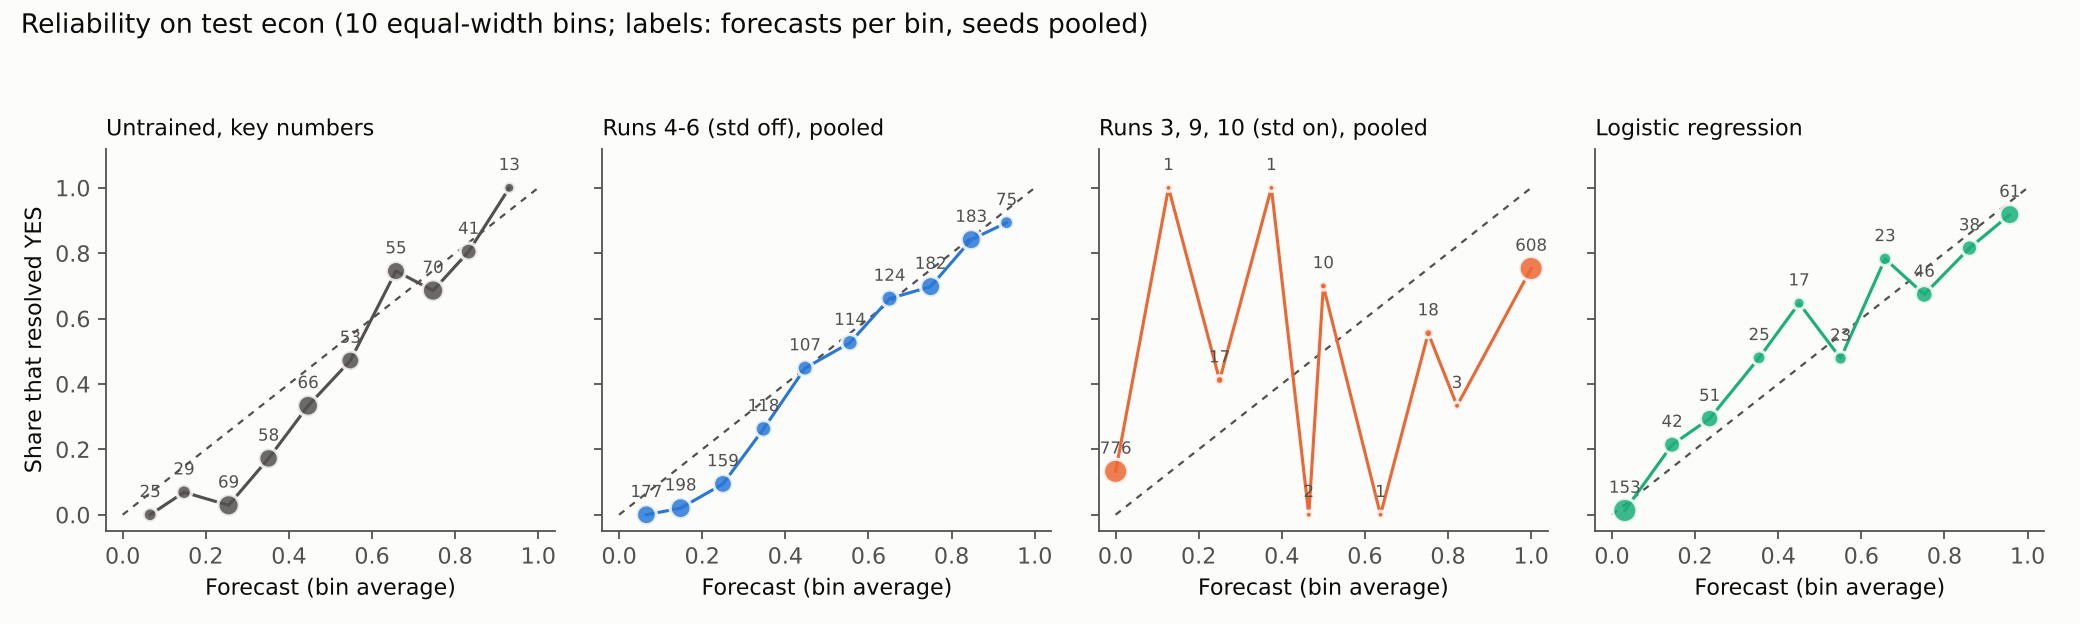
\includegraphics[width=\linewidth]{figures/reliability_test.png}
\caption{Reliability diagrams on test econ, as in Figure~\ref{fig:reliability}. Runs 4--6 sit below the diagonal between about 0.1 and 0.4: they forecast YES too often for the test period.}
\label{fig:reliability_test}
\end{figure}

\needspace{0.62\textheight}
\section{Test-split timeline}
\label{app:timeline}

All times are U.S. Eastern, 2026; commits are in the public repository, and the plan's own record of each change is in \texttt{eval/test\_plan.md}.

\begin{table}[H]
\centering\small
\begin{tabularx}{\linewidth}{@{}llX@{}}
\toprule
When & Commit & Event \\
\midrule
28 Oct, 22:14 & -- & First dry runs of the test notebook. They pair made-up model answers with the real baselines, so they compute and print the baselines' test scores (market price, base rate, rules, logistic regression). Dry runs continued through the revisions below. \\
29 Oct, 08:06 & \texttt{17b601b} & Plan and test notebook first committed. The plan stated, wrongly, that no baseline had been scored. \\
29 Oct, 08:25 & \texttt{f113ac1} & Amendment 1: P2 and S3 include run 10; P3's second criterion changed because validation run 10 did not meet the original one. \\
29 Oct, 08:57 & \texttt{10b109c} & Amendment 2: gradient-boosted trees (S8) added after a reviewer asked for a stronger baseline; settings chosen by cross-validation on the training questions. \\
29 Oct, 12:10 & \texttt{ba3e6ef} & Amendment 3, after an outside review: announcement-level intervals; wording of the aggregation rule, scored population, timing audit and failure handling. No prediction or threshold changed. \\
29 Oct, 12:45 & \texttt{ba3e6ef} & The loading check run alone on Kaggle: every model answered 80 validation questions; no test question was scored. \\
29 Oct, 13:26--13:38 & -- & Last dry runs: the notebook, the trees script in test mode (computing the trees' test scores) and the verdict script, all with made-up model answers. \\
29 Oct, 15:12 & \texttt{7e515ef} & Amendment 4: the baseline exposure disclosed; verdict script and the trees' test mode added; P3's wording matched to how it is computed. No prediction or threshold changed. \\
30 Oct, 20:28 & \texttt{7e515ef} & The scored run: the models' first answers to test questions. \\
30 Oct, 23:47 & \texttt{f35629a} & Results committed. \\
\bottomrule
\end{tabularx}
\end{table}

No language model answered a test question before the scored run. The baselines' test scores were available from the first dry run on, before the plan was first committed and before amendments 1 to 3, so they could have been seen when those amendments were made. The amendments' stated reasons are validation results and outside reviews, and every baseline's settings were fixed on training questions only.

\section{Brier skill scores}
\label{app:skill}

\begin{table}[H]
\centering\small
\caption{Brier skill relative to the base rate: $1 - \text{Brier}/\text{Brier}_{\text{base rate}}$. Negative means worse than the base rate.}
\begin{tabular}{lccc}
\toprule
Method & Validation econ & Test econ & Held-out weather \\
\midrule
Market price & 0.747 & 0.704 & 0.274 \\
Gradient-boosted trees, key numbers + series & 0.378 & 0.494 & $-0.416$ \\
Logistic regression, key numbers & 0.331 & 0.475 & $-0.441$ \\
Counting rule & 0.311 & 0.442 & $-0.574$ \\
Runs 4--6 (key numbers, std off) & 0.296 to 0.306 & 0.408 to 0.455 & $-0.498$ to $-0.605$ \\
Untrained, key numbers & 0.172 & 0.334 & $-0.606$ \\
Runs 3, 9, 10 (key numbers, std on) & 0.082 to 0.131 & 0.217 to 0.282 & $-0.876$ to $-1.145$ \\
Latest-result rule & 0.103 & 0.220 & $-1.120$ \\
Run 8 (shuffled outcomes) & 0.030 & 0.085 & $-0.606$ \\
Runs 1, 7 (plain prompt) & $-0.098$, $-0.081$ & 0.019, $-0.072$ & $-0.829$, $-1.093$ \\
Untrained, plain prompt & $-0.119$ & $-0.070$ & $-1.060$ \\
\bottomrule
\end{tabular}
\end{table}

\section{Stated probabilities at the start and end of training}

\begin{figure}[H]
\centering
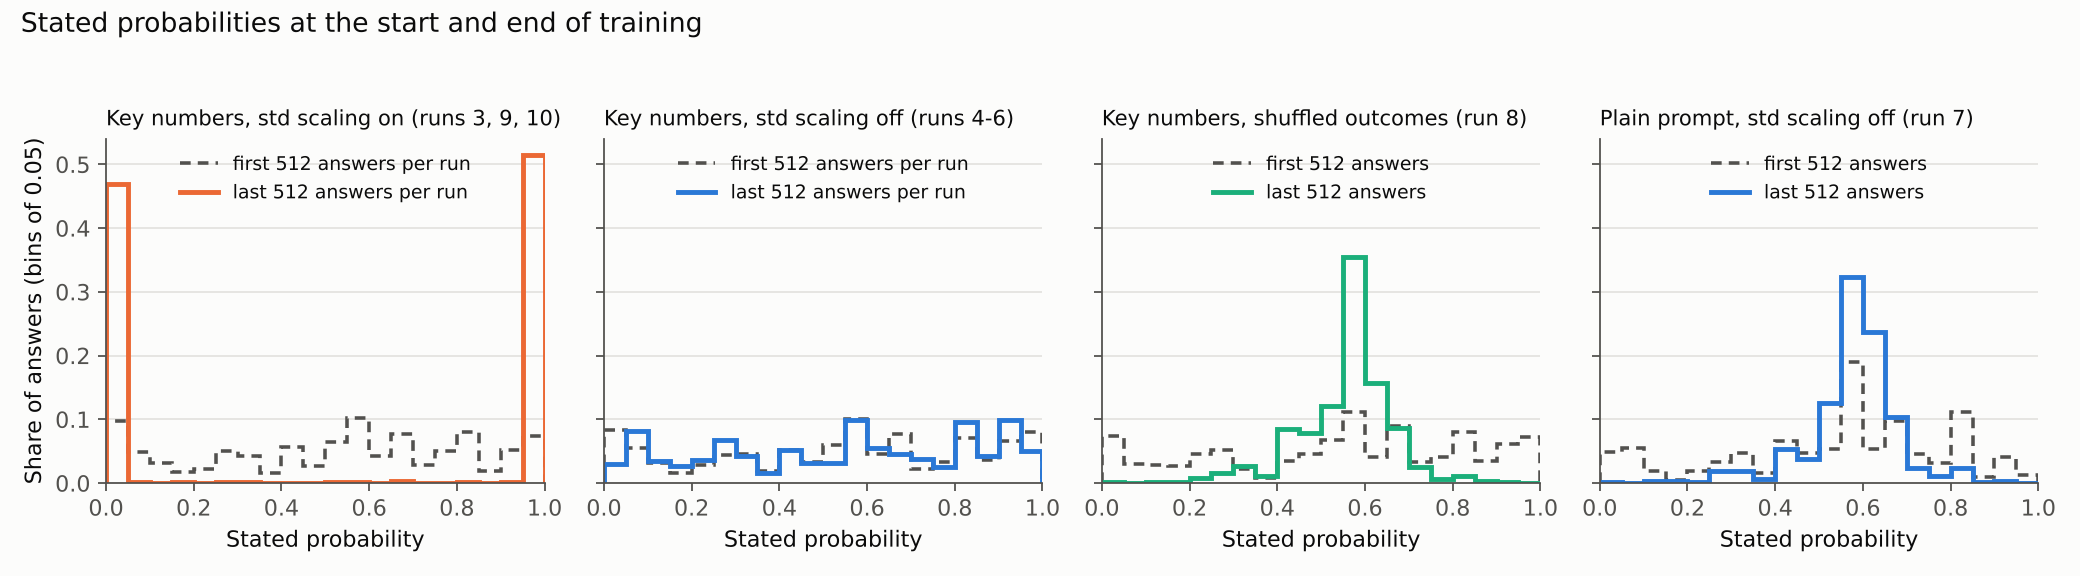
\includegraphics[width=0.88\linewidth]{figures/probability_histograms.png}
\caption{Stated probabilities in the first and last 512 training answers of each run (seeds pooled).}
\label{fig:hist}
\end{figure}

\section{Issues found during the project}

\texttt{writeup/hacks.md} in the repository has the full log. Each issue changed what the reward or a metric measured, but they are of three different kinds.
\begin{itemize}[leftmargin=*]\raggedright
\item \textbf{Parser defect.} The answer ``\texttt{Probability:~8/17~=~0.47}'' was read as 8 and rejected. We now parse the last number on the last probability line.
\item \textbf{Metric artifacts.}
  \begin{itemize}
  \item A lower average forecast looked like a held-out gain (run 1 on weather); AUC and a shift-matched baseline catch it.
  \item The yes-minus-no gap on training answers grows with sharpening alone, so we judge runs on held-out AUC.
  \end{itemize}
\item \textbf{Optimizer failures.}
  \begin{itemize}
  \item Overconfidence with more training (run 2, std scaling on).
  \item Collapse onto the latest-result rule (runs 3, 9 and 10), absent with std scaling off.
  \end{itemize}
\end{itemize}

\end{document}
